\documentclass{report}

%% Language and font encodings
\usepackage[english]{babel}
\usepackage[utf8x]{inputenc}
\usepackage[T1]{fontenc}

%% Sets page size and margins
\usepackage[top=3cm,bottom=2cm,left=3cm,right=3cm,marginparwidth=1.75cm]{geometry}

%% Useful packages
\usepackage{amsmath}
\usepackage{graphicx}
\usepackage[colorinlistoftodos]{todonotes}
\usepackage[colorlinks=true, allcolors=black]{hyperref}

% Specify bibliography package
\usepackage{natbib}



\title{Print-A-Pal \linebreak User Manual}
\author{MD Rashad \& Lokesh Podipireddy}
\date{\vfill April 2017}



\begin{document}

\maketitle

\tableofcontents

\chapter{Revision History}
\section{Revision 0}
Initial User Manual compiled.
\section{Revision 1} Changes to core 2D canvas components.
\section{Revision 2} Changes to design functions.
\section{Revision 3} Description and organization changes.


% For each day of class, you will have a new chapter
\chapter{Introduction}

% You should have one section per assigned reading
\section{About Print-A-Pal}
Print-A-Pal was founded by Lokesh and MD, two computer science students taking the Capstone course in which students are required to create an innovative technology project highlighting our knowledge and creative drive.  We chose an idea that involved the perfect mix of software and art, and created a creative studio to turn virtual imaginations to real life.  
 
\section{What does Print-A-Pal Do?}

Print-a-Pal is online application that takes a 2D picture and creates a 3D rendering of that drawing which can be later saved as an STL file for 3D printing. Print-a-Pal allows the user the manipulate 3D object by manipulating the 2D drawing itself. This is done by limiting the user to certain 2D drawing shapes and manipulating those shapes in 2D space to manipulate the 3D model. As the user manipulates a 2D shape, the 3D model updates as well accordingly. This type of system allows the user to learn the system quickly.

\section{About this manual}

This document will be introducing the basic overview of the web application with specific concentration towards the use of the drawing application. It Specifies the major features that are essential to build a robust 3D model and states how to correctly use these features. 

\chapter{Setting up}
\section{How to run Print-A-Pal}
Print-A-Pal actually works directly in your web browser! As long as WebGL is enabled, just head to printapal.io.
\subsection{Setting up WebGL in your browser}
As of now, WebGL is only available for Chrome, Firefox, and Safari.
\subsubsection{Google Chrome}
\begin{itemize}
  \item Go to "chrome://settings"
  \item Click the "+Show advanced settings" button
  \item In the "System" section, ensure the "USe hardware acceleration when available" checkbox is checked (you'll need to relaunch Chrome for changes to take effect)
  \item Go to "chrome://flags"
  \item Ensure that "Disable WebGL" is not activated (you will need to relaunch again for it to register) 
\end{itemize}
Then check if it worked:
\begin{itemize}
    \item go to "chrome://gpu" 
    \item Inspect the "WebGL" item in the "Graphics Feature Status" list.  
    \begin{itemize}
    \item If the status reads "Hardware accelerated", WebGL is enabled and running on the graphics card
    \item If the status reads "Software only, hardware acceleration unavailable, WebGL is enabled but running in software.
    \item If it reads "Unavailable", WebGL isn't running in hardware or software
    \end{itemize}  
\end{itemize}
\subsubsection{Mozilla Firefox}
\begin{itemize}
	\item Go to "about: config"
	\item Search for "webgl.disabled"
    \item Ensure that its value is false
\end{itemize}
Then check if it worked:
\begin{itemize}
	\item Go to "about:support"
	\item Inspect the "WebGL Renderer" row in the "Graphics" table:
    \begin{itemize}
    	\item If the status reads the name of your gpu, WebGL is working
        \item If the status reads something like "Blocked for your graphics card because of unresolved driver issues", your gpu is blacklisted
    \end{itemize}
\end{itemize}
\subsubsection{Safari}
\begin{itemize}
	\item Go to "Preferences"
    \item Select "Advanced" tab
    \item Ensure that the "Show Develop menu in menu bar" box is checked
    \item In "Develop" menu, ensure "Enable WebGL" is checked
\end{itemize}

\chapter{Instructions on using application}
\section{Sign up and Login}

\subsection*{Sign up}

\paragraph{} In order to sign up for this service, you must to www.printapal.io/signup and enter the fields shown below.

\paragraph{figure 1.}
\begin{center}
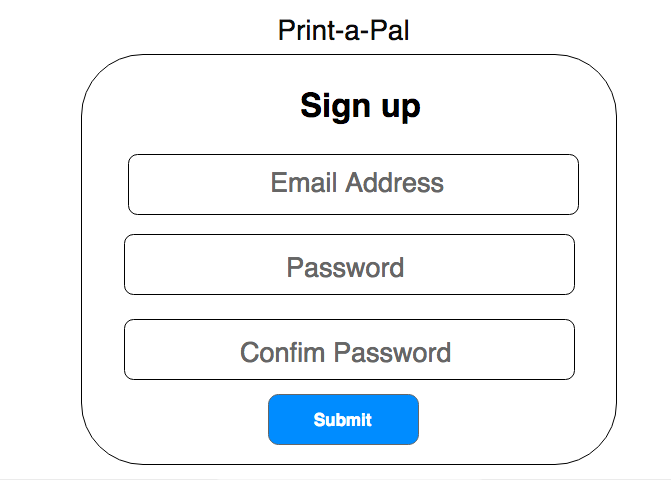
\includegraphics[width=\textwidth/2]{sign_up.png}
\end{center}

\paragraph{} Once this has gone through successfully, you will receive and email which has an activation link for your account. Once this email link has been clicked, it will you take you to your profile page. You can edit your profile by clicking the pencil icon. You can start a new project or browse old ones as well. The next section explains how the drawing module works. 
\paragraph{figure 2.}
\begin{center}
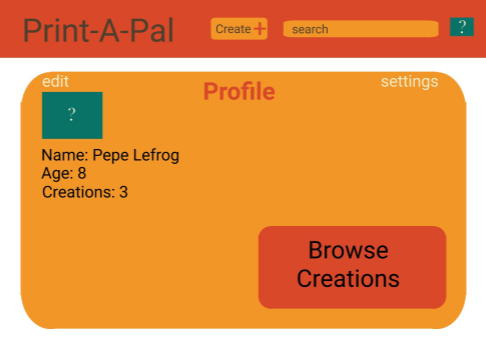
\includegraphics[width=\textwidth/2]{profile.png}
\end{center}

\section{Drawing Project Application}

\paragraph{} The drawing application is where the user creates their 3D model. The window is split in two parts. The screen on the left hand side is the 2D drawing space. In this space there are two modes: draw mode and model mode. Draw mode is where user first creates their 2D drawing using the pencil and line tool. Additionally the user also has the option to upload an image of their choice for draw mode. {}

\paragraph{} Once the user has drawn their initial drawing or has an image uploaded to draw mode, they can click next and move on to model mode. Model mode is where the user uses two basic shapes to create three models. Model mode works by creating an overlay on top of the initial drawing that is just transparent enough to be able trace the basic shapes over the initial drawing. The figure below shows how it is setup.
\paragraph{figure 3.}
\begin{center}
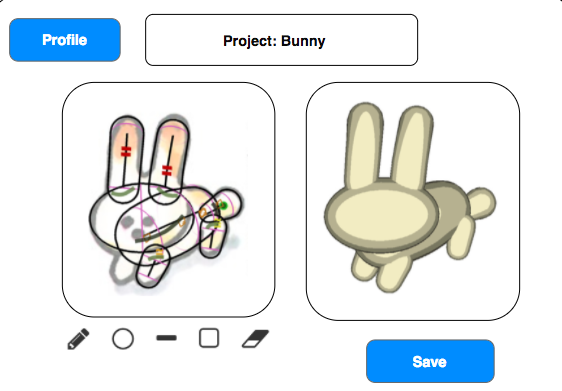
\includegraphics[width=\textwidth/2]{draw_page.png}
\end{center}
\paragraph{} As you can can see, the user drew a bunny in draw mode. Now in model mode, the user is tracing parts of the bunny's body with ovals and circles. The user is only allowed to use these two shapes in model mode but they are allowed to manipulate these shapes as the please to fit the 3D model properly.

\paragraph{} There are multiple handles to manipulate these basic shapes to acquire the desired 3D shape. Each handle serves a specific purpose with respects to the 3D output. 

\subsection*{Ovals}

\paragraph{} Ovals are one of the two basic shapes that will be used to create a 3D model. An oval represents a cylinder in 3D space but the cylinder can be bent like a curve, it can be scaled in any direction and can be connected to other 3D objects in a variety of ways. 

\paragraph{figure 4.}
\begin{center}
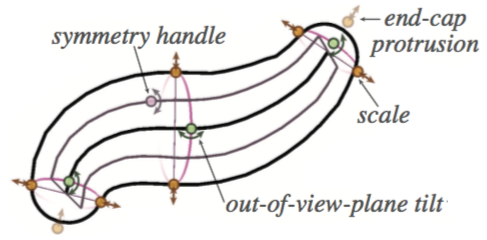
\includegraphics[width=\textwidth/2]{oval_handles.png}
\end{center}

\subsection*{Ovals: End-cap Protrusion}

\paragraph{} The end-cap protrusion handle is responsible for the roundedness and length of the ends of the cylinder. This is done by dragging the handle either away from the spine to make it more round or towards the spine to make it more flat.

\subsection*{Ovals: Out-of-view-plane Tilt}

\paragraph{} The application assumes a 2D x,y plane for the drawing modeling mode. The positive z-direction is towards the user. The out-of-view-plane tilt handle is responsible for getting parts of the objects to lean more towards the positive or negative z-axis. The way to use this handle is to click on the handle and a pop-up will appear that will display the current level of tilt which is set to 0. The user will click the plus button to tilt the object towards the user and negative for tilt away from the user. The 3D model will be updated each time the user clicks either the plus or minus button. There are three locations for this handle along the spine. One in the middle and two and the either ends of the spine.

\subsection*{Ovals: Scale}

\paragraph{} The scale handle is responsible scaling the oval which in turn will scale the 3D cylinder. This is done dragging the scale handle perpendicular to the spine. towards the spine will shrink while away from the spine will make it bigger. There are 6 handles in total. These handles will exist in pairs of two. Each pair will be present on the opposite sides of the oval and the pairs exist on the edge of the oval parallel to the spine. Two pairs on either end and a pair in the middle.

\subsection*{Circles}

\paragraph{} Unlike Ovals, circles have a less functionality when it comes to manipulation but nonetheless, it is required to properly create 3D models. circles represent spheres in 3D space and consist of three handles. You can control its orientations, its radius and its tilt relative to the z-axis.
\paragraph{} 
\subsection*{Circles: Orientation and Size}

\paragraph{} The orientation and size handle is responsible for manipulating the size and orientation of the sphere. The rotation is done by rotating the dot about its axis using the mouse while the size is adjusted by pulling the handle up or down to increase or decrease in size respectively.

\subsection*{Ovals: Out-of-view-plane Tilt}

\paragraph{} The Out-of-view-plane Tilt works exactly as the one for ovals. You can change the tilt towards the positive and negative z-directions by hitting the plus or minus buttons. The difference between the oval and circle is that there is only handle for out-of-view-plane tilt while the oval has 3.

\paragraph{figure 5.}
\begin{center}
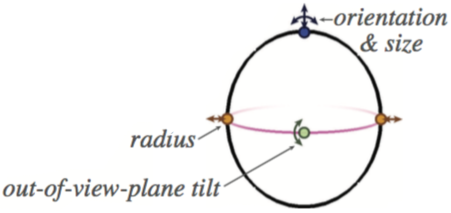
\includegraphics[width=\textwidth/2]{sphere_handles.png}
\end{center}

\subsection*{Shape Configurations}

\paragraph{} Shapes configurations are responsible adjusting the shapes that are either too complicated or impossible to implement using handles. There are many configurations the application offers to adjust your shapes more appropriately. Below are some of the configurations

\subsection*{Alignment Configuration}

\paragraph{} Alignment configurations are responsible for aligning a shape with respect to another shape. For example, if you have two shapes, you can position on in front of the other, merge them both or put the behind the other shape. Below is an example of this configuration. The green connection means put the shape in front while the black means put the shape in the back. the rotation of the link represents the angle it should be positioned under. The alignment tool can found on the left hand menu under configurations. You must select the shape before select the configuration you would like to perform.

\paragraph{figure 6.}
\begin{center}
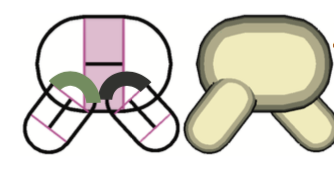
\includegraphics[width=\textwidth/2]{align_config.png}
\end{center}

\subsection*{Same Length Configuration}

\paragraph{} Same length configurations are responsible for the match the length and shape of two different shapes. Below is an example of this configuration. The same length tool can be found on the left hand menu under configurations. You must select the shapes before selecting the configuration you would like to perform.

\paragraph{figure 7.}
\begin{center}
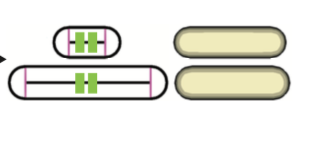
\includegraphics[width=\textwidth/2]{same_length2.png}
\end{center}

\chapter{Definitions and Key components}

% You should have one section per assigned reading
\begin{itemize}
	\item Configurations
    \begin{itemize}
    	\item Configurations are additional operations to manipulate your shape. They can be found in the menu on the left hand side of the drawing screen.
    \end{itemize}
    \item Handles
    \begin{itemize}
    	\item handles are little notches that found on the basic 2D shapes. Each handle serves a different purpose in terms of manipulating the 3D object. See the Drawing application section for more information 
    \end{itemize}
    \item Out-of-view-plane tilt
    \begin{itemize}
    	\item This is a special operation. What it does is that tilts a section of the 3D model either towards the user or away from the user. When applying this handle, you can see how it impacts the 3D model immediately.
    \end{itemize}
    \item WebGL
    \begin{itemize}
    	\item This is a graphics library that is responsible for displaying 3D objects onto your browser.
    \end{itemize}
\end{itemize}



\chapter{Frequently Asked Questions}
\begin{itemize}
	\item What do I need to use Print-A-Pal?
    \begin{itemize}
    	\item You just need to access printapal.io on Chrome, Firefox, or Safari and ensure WebGL is enabled
    \end{itemize}
    \item Will my old creations be saved?
    \begin{itemize}
    	\item As long as you are signed in to your account, any previous projects can be saved to your account.
    \end{itemize}
    \item How old do I have to be to use Print-A-Pal?
    \begin{itemize}
    	\item As long as you know how to use a computer you can print your own pal!	
    \end{itemize}
\end{itemize}
\end{document}












